\documentclass[aspectratio=169, 11pt]{beamer}

% --- Theme ---
\usetheme{metropolis}
\usepackage{booktabs}
\usepackage{graphicx}
\usepackage{xcolor}

% Muted blues/grays palette
\definecolor{primary}{HTML}{2c3e50}
\definecolor{accent}{HTML}{2980b9}
\definecolor{alert}{HTML}{c0392b}
\setbeamercolor{frametitle}{bg=primary, fg=white}
\setbeamercolor{progress bar}{fg=accent}

% Figure path
\graphicspath{{../output/diagnostics/}}

% --- Metadata ---
\title{Global Valuation --- Data Exploration}
\subtitle{Schema, Coverage, and Preliminary Diagnostics}
\author{Augustin Landier}
\institute{HEC Paris}
\date{February 2026}

\begin{document}

\maketitle

% ===================================================================
\section{Data Overview}
% ===================================================================

\begin{frame}{Datasets}
\begin{table}
\centering
\small
\begin{tabular}{@{}llrrp{5.5cm}@{}}
\toprule
\textbf{File} & \textbf{Size} & \textbf{Rows} & \textbf{Cols} & \textbf{Description} \\
\midrule
\texttt{compustat\_global}   & 2.3 GB & 981K   & 468 & Global annual fundamentals (124 countries) \\
\texttt{compustat\_america}  & 0.8 GB & 254K   & 984 & NA fundamentals + CRSP link \\
\texttt{returns\_global}     & 1.9 GB & 10.4M  &  25 & Global monthly prices \\
\texttt{returns\_america}    & 0.9 GB & 3.6M   &  55 & CRSP US monthly returns \\
\bottomrule
\end{tabular}
\end{table}

\vspace{0.3cm}
\begin{itemize}
\item Compustat Global: fiscal years 1987--2025
\item Compustat America: fiscal years 1986--2025
\item Returns America: 1986--2024, Returns Global: 2007--2026
\end{itemize}
\end{frame}

% ===================================================================
\section{Coverage}
% ===================================================================

\begin{frame}{Top 20 Countries by Firm-Years (Compustat Global)}
\centering
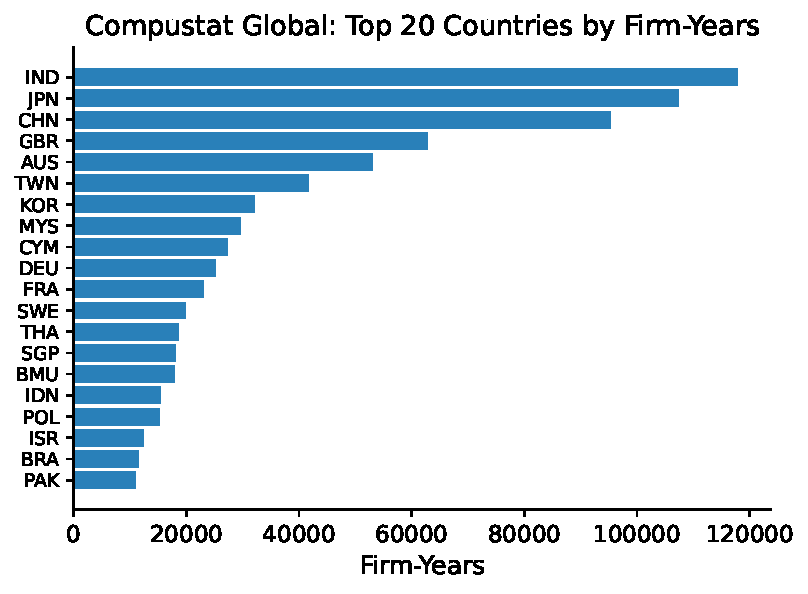
\includegraphics[width=0.85\textwidth]{coverage_by_country.pdf}
\end{frame}

\begin{frame}{Coverage Over Time}
\centering
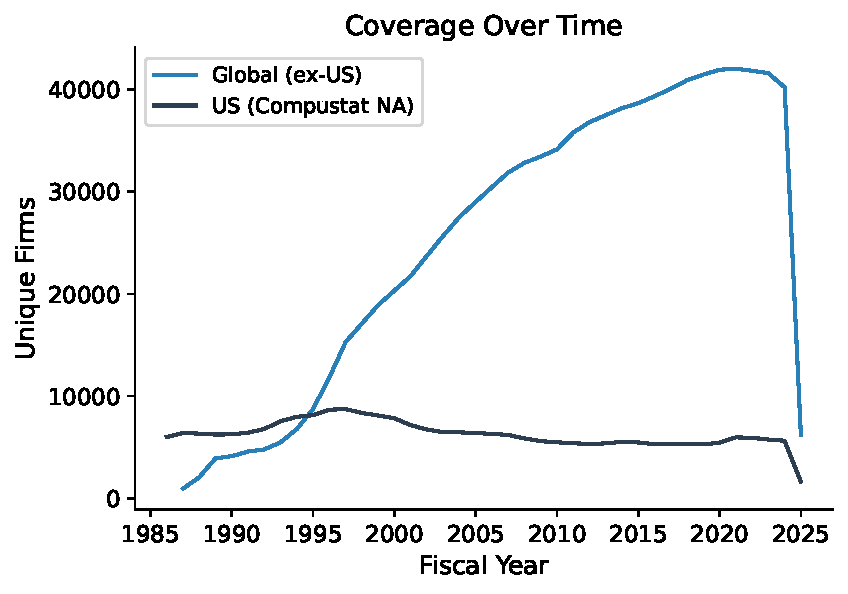
\includegraphics[width=0.85\textwidth]{coverage_by_year.pdf}

\vspace{0.2cm}
\small Global coverage peaks at $\sim$41K firms (2022); US stable at $\sim$5--8K.
\end{frame}

% ===================================================================
\section{Key Variables}
% ===================================================================

\begin{frame}{Missingness (\% NaN)}
\begin{columns}[T]
\begin{column}{0.48\textwidth}
\textbf{Compustat Global}
\begin{table}
\centering
\small
\begin{tabular}{@{}lr@{}}
\toprule
Variable & \% Missing \\
\midrule
\texttt{at} (assets)   &  0.3\% \\
\texttt{ceq} (equity)  &  0.4\% \\
\texttt{sale}          & 18.3\% \\
\texttt{ebitda}        &  1.2\% \\
\texttt{mkvalt}        & \textcolor{alert}{not in file} \\
\bottomrule
\end{tabular}
\end{table}
\end{column}
\begin{column}{0.48\textwidth}
\textbf{Compustat America}
\begin{table}
\centering
\small
\begin{tabular}{@{}lr@{}}
\toprule
Variable & \% Missing \\
\midrule
\texttt{at} (assets)   &  8.4\% \\
\texttt{ceq} (equity)  &  8.5\% \\
\texttt{sale}          &  8.8\% \\
\texttt{ebitda}        & 11.4\% \\
\texttt{prcc\_f}       &  0.4\% \\
\texttt{csho}          &  0.6\% \\
\bottomrule
\end{tabular}
\end{table}
\end{column}
\end{columns}

\vspace{0.4cm}
\small
\textbf{Note:} \texttt{mkvalt} absent from Global file --- market cap must be computed by merging with \texttt{returns\_global} (price $\times$ shares).
\end{frame}

% ===================================================================
\section{Data Quality}
% ===================================================================

\begin{frame}{Data Quality Flags}
\begin{columns}[T]
\begin{column}{0.48\textwidth}
\textbf{Compustat Global}
\begin{table}
\centering
\small
\begin{tabular}{@{}lr@{}}
\toprule
Flag & Count \\
\midrule
Zero total assets     &  7,242 \\
Negative total assets &      4 \\
Negative equity       & 33,321 \\
\bottomrule
\end{tabular}
\end{table}
\end{column}
\begin{column}{0.48\textwidth}
\textbf{Compustat America}
\begin{table}
\centering
\small
\begin{tabular}{@{}lr@{}}
\toprule
Flag & Count \\
\midrule
Zero total assets     &     20 \\
Negative total assets &      0 \\
Negative equity       & 10,339 \\
\bottomrule
\end{tabular}
\end{table}
\end{column}
\end{columns}

\vspace{0.4cm}
\begin{itemize}
\item Negative equity: 3.4\% of Global, 4.1\% of US --- must filter for P/B
\item Zero-asset firms likely shell companies or data errors
\end{itemize}
\end{frame}

% ===================================================================
\section{Valuation Distributions}
% ===================================================================

\begin{frame}{P/B Distributions: Raw vs Winsorized}
\centering
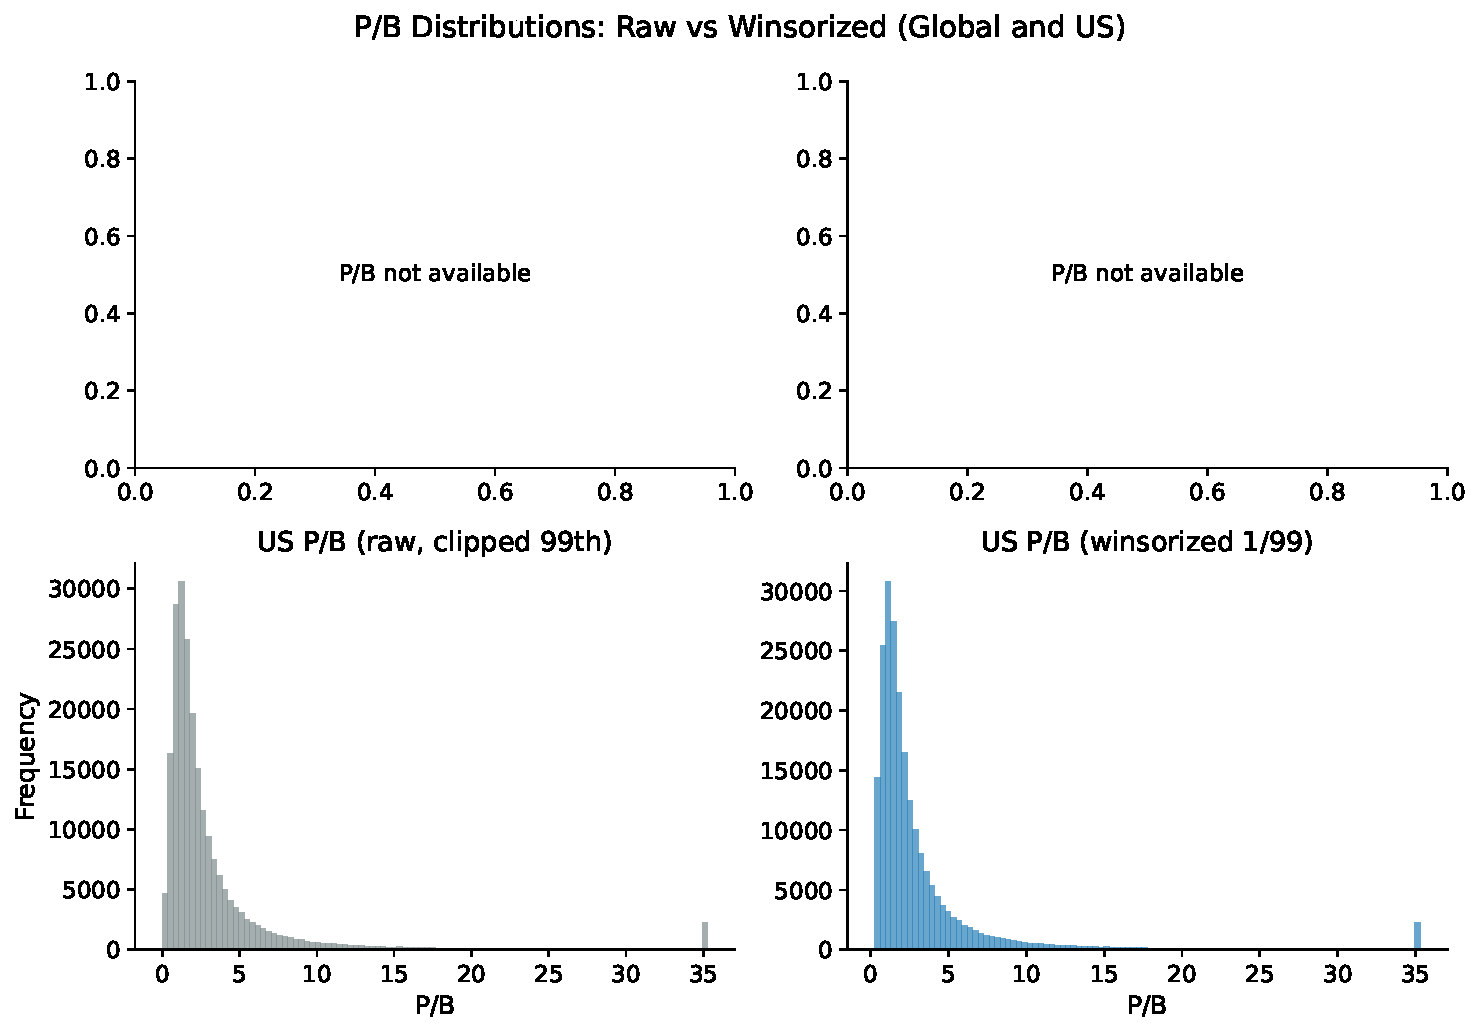
\includegraphics[width=0.82\textwidth]{valuation_distributions.pdf}

\vspace{0.2cm}
\small Global P/B unavailable (no \texttt{mkvalt}). US P/B: heavy right tail tamed by 1/99 winsorization.
\end{frame}

% ===================================================================
\section{Returns}
% ===================================================================

\begin{frame}{Returns Summary}
\begin{columns}[T]
\begin{column}{0.48\textwidth}
\textbf{Returns America (CRSP)}
\begin{table}
\centering
\small
\begin{tabular}{@{}lr@{}}
\toprule
Statistic & Value \\
\midrule
Unique securities & 33,074 \\
Date range        & 1986--2024 \\
Non-missing \texttt{RET} & 98.5\% \\
Mean monthly      & 0.91\% \\
Median monthly    & 0.19\% \\
Std dev           & 18.3\% \\
\bottomrule
\end{tabular}
\end{table}
\end{column}
\begin{column}{0.48\textwidth}
\textbf{Returns Global}
\begin{table}
\centering
\small
\begin{tabular}{@{}lr@{}}
\toprule
Statistic & Value \\
\midrule
Unique securities & 58,261 \\
Date range        & 2007--2026 \\
Return column     & \textcolor{alert}{none} \\
Price column      & \texttt{prccm} \\
\bottomrule
\end{tabular}
\end{table}

\vspace{0.3cm}
\small Returns must be computed from monthly prices.
\end{column}
\end{columns}
\end{frame}

% ===================================================================
\section{Key Takeaways}
% ===================================================================

\begin{frame}{Pitfalls and Next Steps}
\textbf{Pitfalls identified:}
\begin{enumerate}
\item \texttt{gvkey} is lowercase in Global, \textbf{uppercase} (\texttt{GVKEY}) in America
\item \texttt{mkvalt} only in America --- Global needs price $\times$ shares merge
\item Returns Global has \textbf{no return column} --- compute from \texttt{prccm}
\item 43K negative-equity observations to handle for P/B ratios
\item Max US monthly return = 3,900\% --- outlier screening needed
\end{enumerate}

\vspace{0.4cm}
\textbf{Next steps:}
\begin{enumerate}
\item Build cleaning pipeline (filter, winsorize, harmonize identifiers)
\item Merge Compustat with returns for market-cap-based ratios
\item Compute country-level valuation multiples (P/B, EV/EBITDA)
\end{enumerate}
\end{frame}

\end{document}
